\documentclass[paper=a4, fontsize=11pt]{scrartcl} % A4 paper and 11pt font size

\usepackage{amsmath,amsfonts,amsthm} % Math packages
\usepackage[english]{babel}
\usepackage{graphicx}

\title{Data Mining Assignment 4}
\author{Yulong Yang\\ netid: \textit{yy231}} % Your name


\date{\normalsize\today} % Today's date or a custom date
\begin{document}

\maketitle % Print the title

%%%%%%%%%%%%%%%%
%%%%% Question 1 %%%%%
%%%%%%%%%%%%%%%%
\section*{Question 1}

\paragraph{Sensitivity to outliers} fuzzy c-means should be slightly better than K-means in terms of being affected by outliers. Because the amount of each point contributes to SSE is weighted in fuzzy c-means, and the weight is inversely proportional to the distance between itself and the centroid. Therefore, the effect of an outlier, who is usually very far from the centroid, would be reduced because of its weight is small.

\paragraph{Handling clusters of different sizes and densities} fuzzy c-means would behave similarly to K-means as it does not have a particular method to deal with the size problem.

\paragraph{Non-global shapes} Again, fuzzy c-means does not have any additional handling of non-global shapes than that of K-means, so they would perform similarly in this case too.

%%%%%%%%%%%%%%%%
%%%%% Question 2 %%%%%
%%%%%%%%%%%%%%%%
\section*{Question 2}

\paragraph{(a)} To account for the weighted edges between nodes and their shared neighbors, instead of assigning number of shared neighbors as their similarity, we assign the sum of weights of the shared neighbors. As each shared neighbor has two edges connecting the two nodes respectively, we use the average of the two weights for each edge.

\paragraph{(b)} The advantage of having weights considered is more accurate clustering as now we also look at the weight of each node. However, it brings extra computations, and also we need to consider now a reasonable function to compute the similarity based on weights.

%%%%%%%%%%%%%%%%
%%%%% Question 3 %%%%%
%%%%%%%%%%%%%%%%
\section*{Question 3}

As advantage, DBSCAN can handle clusters with different sizes and shapes; on the other hand, DBSCAN cannot separate overlapped clusters as well as K-means does.

%%%%%%%%%%%%%%%%
%%%%% Question 4 %%%%%
%%%%%%%%%%%%%%%%
\section*{Question 4}

\paragraph{(a)} outliers are marked as below.

\begin{figure}[htbp]
\begin{center}
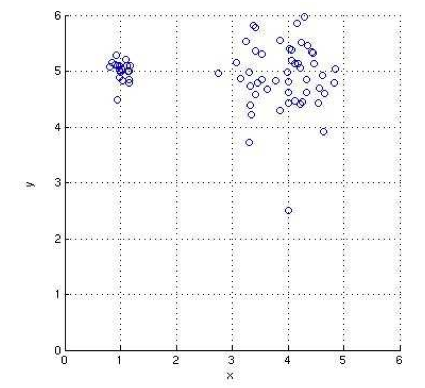
\includegraphics[width=0.5\textwidth]{hw4pic1}
\caption{Outliers}
\label{hw4pic1}
\end{center}
\end{figure}


\paragraph{(b)} If the threshold is 0.5, the 2nd, 4th, 6th, 8th and 9th nodes are all outliers.

\paragraph{(c)} If the threshold is 2.5, the 2nd, 4th and 6th nodes are outliers.

\paragraph{(d)} The distance-based algorithm (kth-nearest neighbor) seems performs worse because some of its outliers are not actual outliers on the graph.

\end{document}